In this section, we explore the statistical and optimization properties of \LipCl networks, and we prove the assumption of~\cite{gouk2021regularisation} that ``adjusting the Lipschitz constant of a feed-forward neural network controls how well the model will generalise to new data''. 
    \vspace{-1mm}
    \subsection{Consistency of \LipCl class}\label{sec:consistency}
  
        \LipCl class enjoys another remarkable property since it is a Glivenko-Cantelli class: minimizers of Lipschitz losses are consistent estimators. In other words, as the size of the training set increases, the training loss becomes a proxy for the test loss: \LipCl neural networks will not overfit in the limit of (very) large sample sizes.  
          
        \begin{restatable}{proposition}{consistenceestimator}{\normalfont\textbf{Train Loss is a proxy of Test Loss}.}\label{thm:consistenceestimator}
            Let $\Prob_{XY}$ a probability measure on $\Xsub\times\Labels$ where $\Xsub\subset\Reals^n$ is a bounded set. Let $(x_i,y_i)_{1\leq i\leq p}$ be a sample of $p$ iid random variables with law $\Prob_{XY}$. Let $\Loss$ be a Lipschitz loss function over $\Reals\times\Labels$. We define:
            \begin{equation}
                \Empirical_p(f)\defeq\frac{1}{p}\sum_{i=1}^p\Loss(f(x_i),y_i)\text{ and }\Empirical_{\infty}(f)\defeq\Expect_{(x,y)\sim \Prob_{XY}}[\Loss(f(x),y)].
            \end{equation}
            Then the empirical loss $\Empirical_p(f)$ converges to the test loss $\Empirical_{\infty}(f)$ (taking the limit $p\rightarrow\infty$):
            \begin{equation}
                \min_{f\in\text{Lip}_L(\Xsub,\Reals)}\Empirical_p(f)\xrightarrow{a.s}\min_{f\in\text{Lip}_L(\Xsub,\Reals)}\Empirical_{\infty}(f).
            \end{equation}
        \end{restatable}
          
        It is another flavor of the bias-variance trade-off in learning. Thanks to Corollary~\ref{thm:zeroerror} we know the \LipCl class does not suffer of bias, while the generalization gap (i.e the variance) can be made as small as we want by increasing the size of the training set (see Figure~\ref{fig:consistency}). The number of examples required to close the generalization gap is dataset specific in general, however it seems that with low $\tau$ fewer examples are required. This result may seem obvious, but we emphasize \textbf{this property is not shared by \LipInf networks} (see Proposition~\ref{thm:lipinfoverfitter} in Appendix~\ref{app:lipinfnotrobust}). Nonetheless, most practitioners take for granted that bigger training sets ensure generalization for \LipInf networks.       
          
        \begin{figure}%[b]
        \centering
        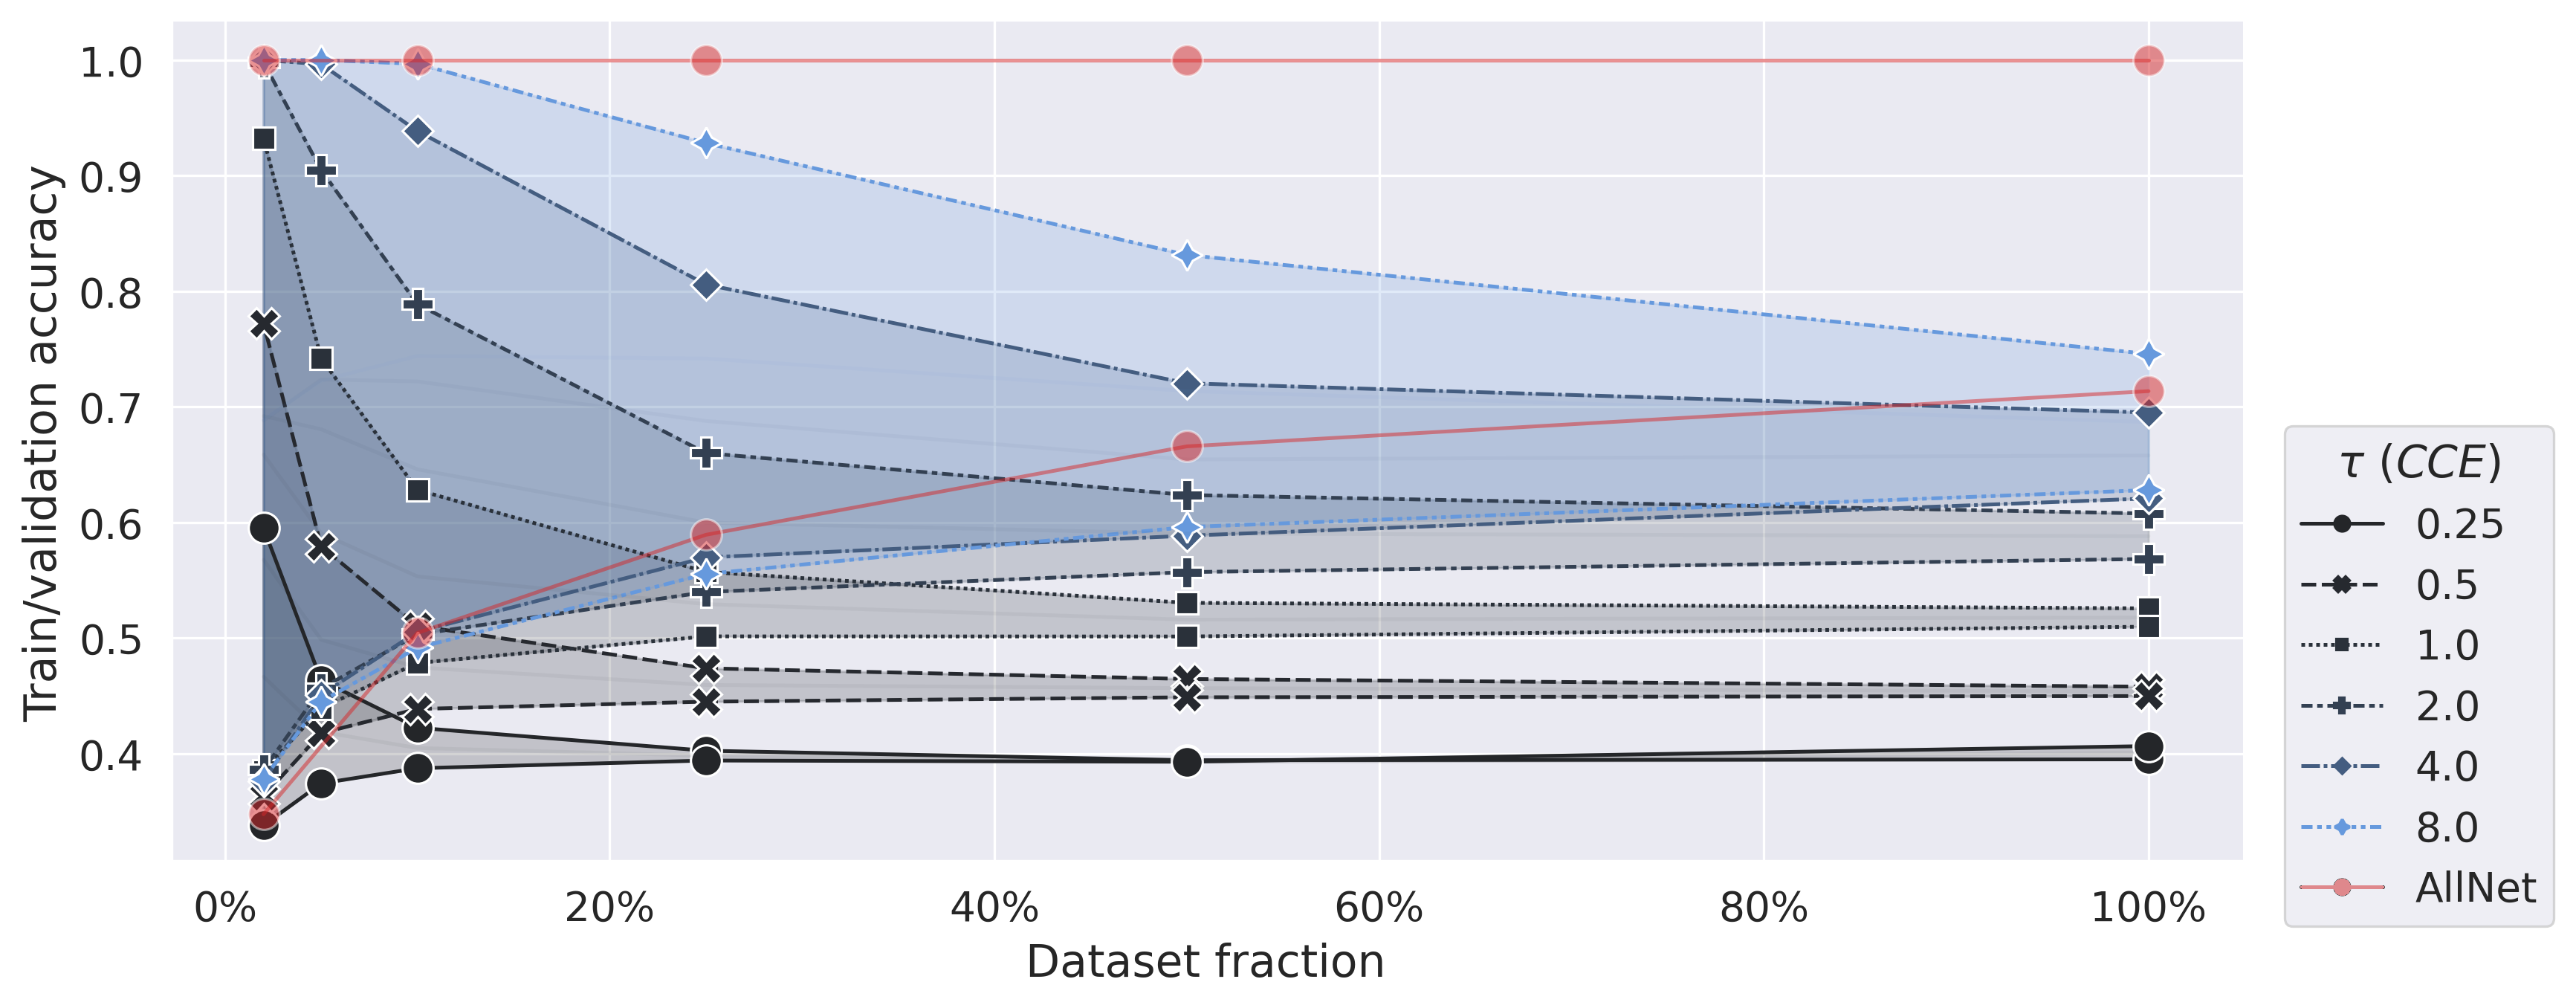
\includegraphics[width=0.9\textwidth]{images/rebuttal/consistency_cifar_up_newlegend.png}
        \caption{\textbf{Link between \LipCl and generalization gap, dataset size and cross-entropy temperature.} We train a CNN on different fractions of the CIFAR10 train set (2\%, 5\%, 10\%, 25\%, 50\% and 100\% on $x$-axis) with different values of temperature $\tau$ (highlighted by different colors). Train (resp. validation) accuracy forms the upper (resp. lower) bound of each envelope. As $\tau$ increases, more samples are required to reduce the generalization gap. Conversely, training a \LipCl network with small $\tau$ is equivalent to training a Lipschitz network with small $L$: the network generalizes well but the accuracy reaches a plateau (under-fitting). The \LipInf network (in red) severely overfit: the generalization gap is large and validation accuracy corresponds to the limit that would reach a \LipCl as $\tau$ increases. See appendix \ref{ap:consistency} for detailed experimental setting.}
        \label{fig:consistency}
        \end{figure}
    
    \subsection{Understanding why unconstrained networks are prone to overfitting}\label{sec:lipinfnotrobust}

        Surprisingly, on $\LipInf$networks, minimization of BCE leads to uncontrolled growth of Lipschitz constant and saturation of the predicted probabilities. This is an impediment to generalization results.     
          
        \begin{restatable}{proposition}{saturatedlimit}{\normalfont\textbf{Optimizing BCE over \LipInf leads to divergence}.}\label{thm:saturatedlimit}
            Let $f_t$ be a sequence of neural networks, that minimizes the BCE over a non-trivial training set (at least two different examples with different labels) of size $p$, i.e assume that:
            \begin{equation}
                \lim_{t\rightarrow\infty}\frac{1}{p}\sum_{i=1}^p\Loss_{\tau}(f_t(x_i),y_i)=0.
            \end{equation}
            Let $L_t$ be the Lipschitz constant of $f_t$. Then $\lim_{t\rightarrow\infty}L_t=+\infty$. There is at least one weight matrix $W$ such that $\lim_{t\rightarrow\infty}\|W_t\|=+\infty$. Furthermore, the predicted probabilities are saturated:
            \begin{equation}
                \lim_{t\rightarrow\infty}\sigma{(f_t(x_i))}\in\{0,1\}.
            \end{equation}
        \end{restatable}   
          
        This issue is especially important since Lipschitz constant and adversarial vulnerabilities are related~\cite{nar2019cross}. The predicted probability $\sigma(f(x))$ will either be $0$ or $1$ (regardless of the train set), which do not carry any useful information on the true confidence of the classifier%, especially in the \textit{out-of-distribution} setting. %For \LipInf networks increasing the size of the training set does not give any formal guarantee to generalization capabilities in general (see Proposition~\ref{thm:lipinfoverfitter} in Appendix).  
        \vspace{-1mm}
        \begin{figure}[ht]
        \begin{minipage}{0.55\linewidth}
        \begin{example}\label{ex:gotcha}%[Illustration on linear classifier]
            Consider a classification task on $\Reals$ with linearly separable inputs $\{-1, 1\}$ and labels $\{-1, 1\}$. We use an affine model $f(x)=Wx+b$ for the logits (with $W\in\Reals$ and $b\in\Reals$) (one-layer neural network). It exists $\bar{W},\bar{b}$ such that $f$ achieves $100\%$ accuracy. However, as noticed in \cite{bishop2006pattern}~(Section~4.3.2) the BCE loss \textit{will not} be zero. The minimization occurs only with the diverging sequence of parameters $(\lambda\bar{W},\lambda\bar{b})$ as $\lambda\rightarrow\infty$. It turns out the infimum is not a minimum!
        \end{example} 
        \end{minipage}
        \begin{minipage}{0.45\linewidth}
        \centering
            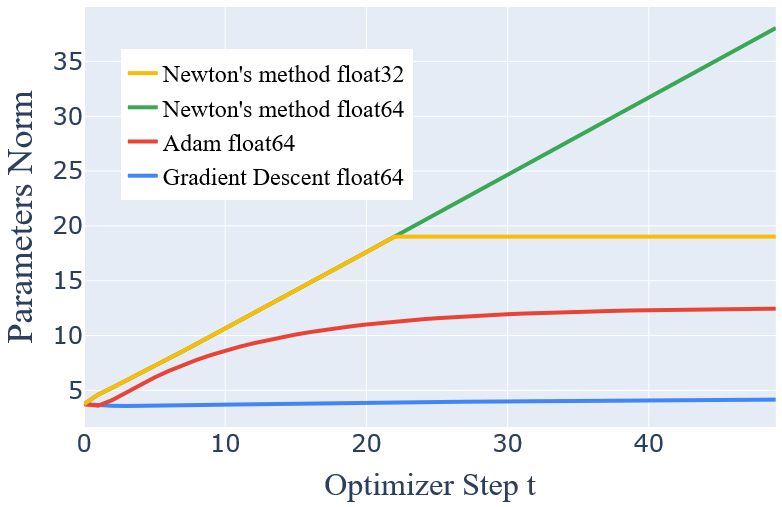
\includegraphics[width=0.9\linewidth]{images/toy/divergence_cropped.png}
            %\captionof{figure}{}
            \caption{}
        \end{minipage}
        \end{figure}
        % \begin{figure}[ht]
        % \centering
        %     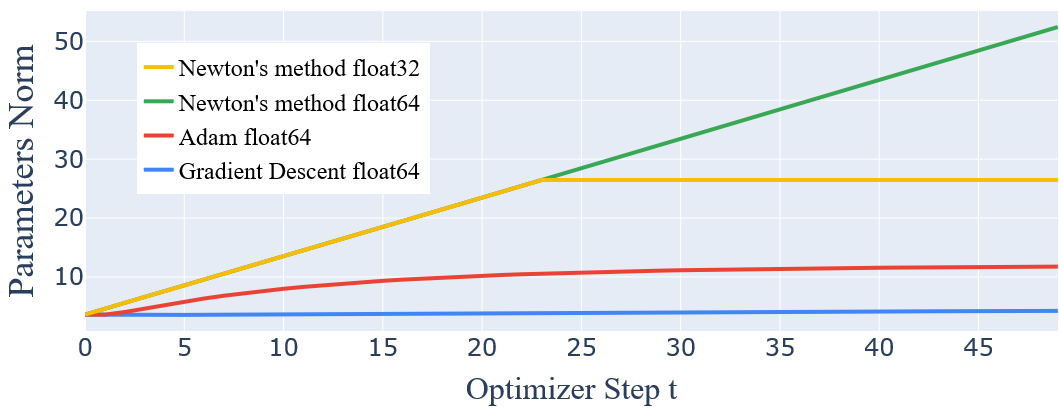
\includegraphics[width=0.65\linewidth]{images/toy/divergence_flat.png}
        %     \caption{
        %         Consider a classification task on $\Reals$ with linearly separable inputs $\{-1, 1\}$ and labels $\{-1, 1\}$. We use an affine model $f(x)=Wx+b$ for the logits (with $W\in\Reals$ and $b\in\Reals$) (one-layer neural network). It exists $\bar{W},\bar{b}$ such that $f$ achieves $100\%$ accuracy. However, as noticed in \cite{bishop2006pattern}~(Section~4.3.2) the BCE loss \textit{will not} be null. The minimization occurs only with the diverging sequence of parameters $(\lambda\bar{W},\lambda\bar{b})$ as $\lambda\rightarrow\infty$. It turns out the infimum is not a minimum!
        %     }
        %     \label{ex:gotcha}
        % \end{figure}
           
        Even on toy example~\ref{ex:gotcha} with a trivial model, the minimization problem is ill-defined. Without weight regularization, the minimizer can not be attained. This is compliant with the high Lipschitz constant of \LipInf networks that have been observed in practice~\cite{scaman2018lipschitz}, and is confirmed by our experiment on MNIST with a ConvNet (see Figure~\ref{fig:divergence}). The spectral norm of the weights is multiplied by 5 over the course of 25 epochs, whereas the validation accuracy remains the same (around 99\%).
          
        Furthermore, there is an issue of vanishing gradients with BCE : first order methods struggle to saturate the logits of \LipInf networks, whereas second order methods in \textit{float64} diverge as expected. The poor properties of the optimizer, and the rounding errors in 32 bits floating point arithmetic, have greatly contributed to the caveat of BCE minimization remaining mostly unnoticed by the community.  
        
    \subsection{Lipschitz classifiers are PAC learnable}
    
        Hinge loss $\Loss^H_m$ and HKR loss $\Loss^{hkr}$ benefit from Proposition~\ref{thm:consistenceestimator}. The certificate $|f(x)|$ can be understood as confidence. Hence, we are interested in a classifier that makes a decision only if the prediction is above some threshold $m>0$, while $|f(x)|<m$ can be understood as examples $x$ for which the classifier is unsure: the label may be flipped using attacks of norm $\epsilon\leq m$. In this setting, we fall back to PAC learnability~\cite{valiant1984theory}: this theory gives bounds on the number of train samples required to guarantee that the test error will fall below some threshold $0\leq e<\frac{1}{2}$ with probability at least $1>\beta\geq 0$, through the use of Vapnik Chervonenkis (VC) dimension bounds~\cite{vapnik2015uniform}.  
          
        \begin{restatable}{proposition}{lipschitzpaclearnable}{\normalfont\textbf{1-Lipschitz Functions with margin are PAC learnable}.}\label{thm:lipschitzpaclearnable}
            Assume $P$ and $Q$ have bounded support $\Xsub$. Let $m>0$ the margin. Let $\Classifiers^m(\Xsub)=\{c^m_f:\Xsub\rightarrow\{-1,\bot,+1\},f\in\text{Lip}_1(\Xsub,\Reals)\}$ be the hypothesis class defined as follow.
            \begin{equation}
                c^m_f(x)=\begin{cases}
                        +1& \text{if } f(x)\geq m,\\
                        -1& \text{if } f(x)\leq -m,\\
                        \bot& \text{otherwise, meaning ``$f$ doesn't feel confident''.}
                \end{cases}
            \end{equation}
                Let $\Ball$ be the unit ball. Then the VC dimension of $\Classifiers^m$ is finite:
                \begin{equation}
                    (\frac{1}{m})^n\frac{vol(\Xsub)}{vol(\Ball)}\leq VC_{\text{dim}}(\Classifiers^m(\Xsub))\leq (\frac{3}{m})^n\frac{vol(\Xsub)}{vol(\Ball)}.
            \end{equation}
        \end{restatable}
          
        Interestingly if the classes are $\epsilon$ separable ($\epsilon>0$), choosing $m=\epsilon$ guarantees that 100\% accuracy is reachable. Prior over the separability of the input space is turned into VC bounds over the space of hypothesis. When $m=0$ the VC dimension of space $\Classifiers^m(\Xsub)$ becomes infinite and the class is not PAC learnable anymore: the training error will not converge to test error in general, regardless of the size of the training set. It is not a contradiction with Proposition~\ref{thm:consistenceestimator}: error $E(c^m_f(x))$ lacks continuity w.r.t $f(x)$ so it is not a consistent estimator.   
          
        This VC bound is \textit{architecture independent} which contrasts with the rest of literature on \LipInf networks. Practically, it means that the \LipCl network architecture can be chosen as big as we want without risking overfitting, as long as the margin $m$ is chosen appropriately. Proposition~\ref{thm:vcdimfullsort} also provides an architecture dependant bound for \LipCl networks. % We also proved an architecture dependant bound $\mathcal{O}\left((n+1)2^W\right)$ for Deel.Lip neural networks of size $W$ over $\Reals^n$ in Appendix~\ref{app:groupsortvcbound}.  
        \begin{restatable}{proposition}{vcdimfullsort}{\normalfont\textbf{VC dimension of \LipCl neural networks}.}\label{thm:vcdimfullsort}
            Let $f_{\theta}:\Reals^n\rightarrow\Reals$ a \LipCl neural network with parameters $\theta\in\Theta$, with \textbf{GroupSort2} activation functions, and a total of $W$ neurons. Let $\Hypothesis=\{\text{sign}f_{\theta}|\theta\in\Theta\}$ the hypothesis class spanned by this architecture. Then we have:
            \begin{equation}
                VC_{\text{dim}}(\Hypothesis)=\mathcal{O}\left((n+1)2^W\right).
            \end{equation}
        \end{restatable}
            
        % From Proposition~\ref{thm:vcdimfullsort} we can derive generalization bounds using PAC theory.
        In literature, tighter VC dimension bounds for neural networks exist, but they assume element-wise activation function~\cite{bartlett2019nearly}. This hypothesis does not apply to GroupSort2 which is known to be more expressive~\cite{tanielian2021approximating}, however we believe that this preliminary result can be strengthened.  

    
        
% \subsection{Experimental results}  %\louis{Ici on déchire tout.} \thib{youhou on est sota sur MNIST.}
      
%     The HKR loss allows to reach SOTA results on certifiable robustness on the Cifar10 dataset with no overhead on the training time. Results are summarized in Table~\ref{tab:hkrsota}.
